\chapter{Image Classification: Data-driven Approach, k-Nearest Neighbor, train/val/test splits}
\section{Image Classification}
\textbf{Motivation.} 
\begin{itemize}
  \item \textbf{Image Classification problem}: the task of assigning an input image one label from a fixed set of categories.
  \item Many other seemingly distinct Computer Vision tasks (such as object detection, segmentation) can be reduced to image classification.
\end{itemize}

\begin{example}
\quad
\end{example}

\begin{figure}[ht]
  \centering
  % Requires \usepackage{graphicx}
  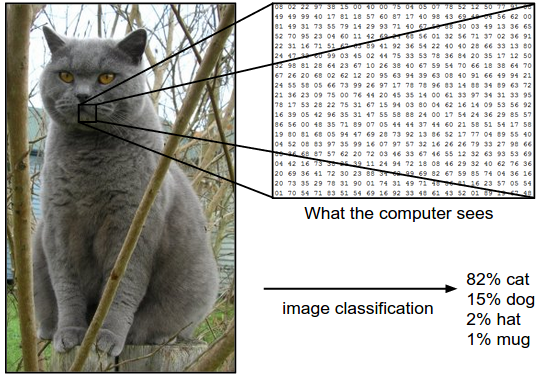
\includegraphics[width=4 in]{pic/classify}\\
  \caption{The task in Image Classification is to predict a single label (or a distribution over labels as shown here to indicate our confidence) for a given image. Images are 3-dimensional arrays of integers from 0 to 255, of size Width $\times$ Height $\times$ 3. The 3 represents the three color channels Red, Green, Blue.}
\end{figure}
  
\textbf{Challenges.} 
\begin{itemize}
  \item \textbf{Viewpoint variation.} A single instance of an object can be oriented in many ways with respect to the camera.
  \item \textbf{Scale variation.} Visual classes often exhibit variation in their size (size in the real world, not only in terms of their extent in the image).
  \item \textbf{Deformation.} Many objects of interest are not rigid bodies and can be deformed in extreme ways.
  \item Occlusion. The objects of interest can be occluded. Sometimes only a small portion of an object (as little as few pixels) could be visible.
  \item \textbf{Illumination conditions.} The effects of illumination are drastic on the pixel level.
  \item Background clutter. The objects of interest may blend into their environment, making them hard to identify.
  \item \textbf{Intra-class variation.} The classes of interest can often be relatively broad, such as chair. There are many different types of these objects, each with their own appearance.
\end{itemize}
\textbf{Note.} As we present (an inexhaustive) list of challenges below, keep in mind the raw representation of images as a 3-D array of brightness values.

A good image classification model must be invariant to the cross product of all these variations, while simultaneously retaining sensitivity to the inter-class variations. 

\begin{figure}
  \centering
  % Requires \usepackage{graphicx}
  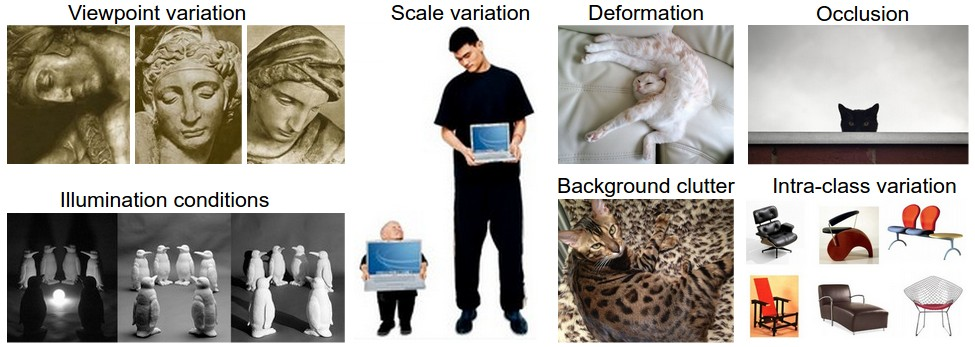
\includegraphics[width=5 in]{pic/challenges}\\
  \caption{Challenges}
\end{figure}

\textbf{Data-driven approach}: provide the computer with many examples of each class and then develop learning algorithms that look at these examples and learn about the visual appearance of each class.
This approach is referred to as a \emph{data-driven approach}, since it relies on first accumulating a \emph{training dataset} of labeled images. 
\quad

\textbf{The image classification pipeline.} 
\begin{itemize}
  \item \textbf{Input}: A set of $N$ images, each labeled with one of $K$ different classes. We refer to this data as the \emph{training set}.
  \item \textbf{Learning}: Using the training set to learn what every one of the classes looks like. We refer to this step as \emph{training a classifier}, or \emph{learning a model}.
  \item \textbf{Evaluation}: Evaluating the quality of the classifier by asking it to predict labels for a new set of images and then compare the true labels of these images to the ones predicted by the classifier, hoping the predictions match up with the true answers (which we call the \emph{ground truth}).
\end{itemize}

\section{Nearest Neighbor Classifier}

Suppose now that we are given the \href{http://www.cs.toronto.edu/~kriz/cifar.html}{CIFAR-10} training set of 50,000 images (5,000 images for every one of the labels), and we wish to label the remaining 10,000.
The nearest neighbor classifier will take a test image, compare it to every single one of the training images, and predict the label of the closest training image. 

\subsection{$L1$ (Manhattan) distance.}
Given two images and representing them as vectors $I_1$, $I_2$, a reasonable choice for comparing them might be the $L1$ distance:
$$d_1(I_1,I_2)=\sum_p|I^p_1-I_2^p|$$
where the sum is taken over all pixels. 
\begin{figure}[ht]
  \centering
  % Requires \usepackage{graphicx}
  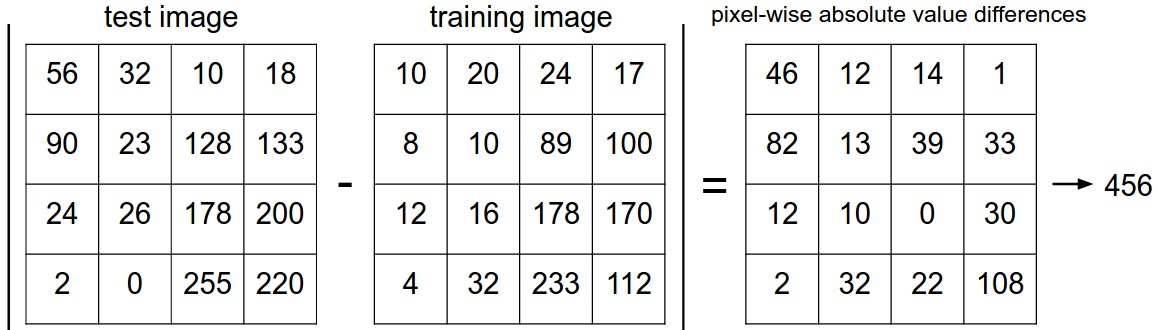
\includegraphics[width=5 in]{pic/nneg}\\
  \caption{An example of using pixel-wise differences to compare two images with L1 distance (for one color channel in this example). Two images are subtracted elementwise and then all differences are added up to a single number. If two images are identical the result will be zero. But if the images are very different the result will be large.}
\end{figure}

\subsection{Implement the classifier in code.}

\subsection{$L2$ (Euclodean) distance.}
Another common choice of computing distances between vectors could be to instead use the $L2$ distance, which has the geometric interpretation of computing the Euclidean distance between two vectors.
$$d_2(I_1,I_2)=\sqrt{\sum_p(I_1^p-I_2^p)^2}$$

\textbf{Note:} In a practical nearest neighbor application we could leave out the square root operation because square root is a \emph{monotonic function}.
That is, it scales the absolute sizes of the distances but it preserves the ordering, so the nearest neighbors with or without it are identical.

\subsection{L1 vs. L2.} 
The $L2$ distance is much more unforgiving than the $L1$ distance when it comes to differences between two vectors. 
That is, the $L2$ distance prefers many medium disagreements to one big one.
$L1$ and $L2$ distances (or equivalently the $L1/L2$ norms of the differences between a pair of images) are the most commonly used special cases of a $p$-norm. 

\section{$k$-Nearest Neighbor Classifier}

\textbf{$k$-Nearest Neighbor Classifier}: Instead of finding the single closest image in the training set, we will find the top $k$ closest images, and have them vote on the label of the test image. 
In particular, when $k = 1$, we recover the Nearest Neighbor classifier. 
Intuitively, higher values of $k$ have a smoothing effect that makes the classifier more resistant to outliers.

\begin{figure}[ht]
  \centering
  % Requires \usepackage{graphicx}
  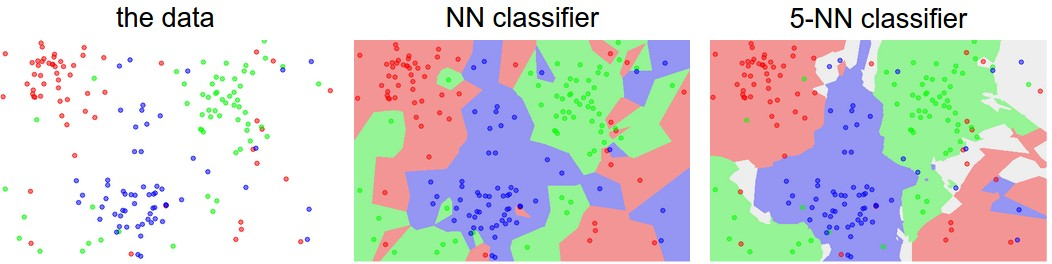
\includegraphics[width=5 in]{pic/knn}\\
  \caption{An example of the difference between Nearest Neighbor and a 5-Nearest Neighbor classifier, using 2-dimensional points and 3 classes (red, blue, green). The colored regions show the decision boundaries induced by the classifier with an $L2$ distance. The white regions show points that are ambiguously classified (i.e. class votes are tied for at least two classes). Notice that in the case of a NN classifier, outlier datapoints (e.g. green point in the middle of a cloud of blue points) create small islands of likely incorrect predictions, while the 5-NN classifier smooths over these irregularities, likely leading to better generalization on the test data (not shown). Also note that the gray regions in the 5-NN image are caused by ties in the votes among the nearest neighbors (e.g. 2 neighbors are red, next two neighbors are blue, last neighbor is green).}
\end{figure}

\section{Validation sets for Hyperparameter tuning}
\subsection{Hyperparameter.}
\begin{itemize}
  \item What $k$ works best in $k$-nearest neighbor classifier? ($k=$?)
  \item What distance function we should use? ($L1$, $L2$ or other choices?)
  \item $\ldots \ldots$
\end{itemize}
These choices are called \textbf{hyperparameters} and they come up very often in the design of many Machine Learning algorithms that learn from data. 

\begin{itemize}
  \item We cannot use the test set for the purpose of tweaking hyperparameters - test set should ideally \textbf{never be touched until one time at the very end}.
  \item \textbf{Overfit} the test set - work well on the test set but significantly reduced performance when deploy the model.
  \item \textbf{Evaluate on the test set only a single time, at the very end.}
\end{itemize}

\subsection{Validation set.}

\textbf{Tuning the hyperparameters}: Split the training set in two: a slightly smaller training set, and what we call a \textbf{validation set}. 

Using CIFAR-10 as an example, we could for example use 49,000 of the training images for training, and leave 1,000 aside for validation. 
This validation set is essentially used as a fake test set to tune the hyper-parameters. 

\textbf{Split your training set into training set and a validation set. Use validation set to tune all hyperparameters. At the end run a single time on the test set and report performance.}

\subsection{Implement in code.}

\subsection{Cross-validation.}

\textbf{cross-validation}: the size of training data (and therefore also the validation data) might be small.

\textbf{Example of cross-validation}: In 5-fold cross-validation, we would split the training data into 5 equal folds, use 4 of them for training, and 1 for validation.
We would then iterate over which fold is the validation fold, evaluate the performance, and finally average the performance across the different folds. 

\subsection{In practice}
\begin{itemize}
  \item People prefer to avoid cross-validation in favor of having a single validation split, since cross-validation can be computationally expensive.
  \item The splits people tend to use is between 50\%-90\% of the training data for training and rest for validation.
  \item Typical number of folds you can see in practice would be 3-fold, 5-fold or 10-fold cross-validation. 
\end{itemize}

\begin{figure}
  \centering
  % Requires \usepackage{graphicx}
  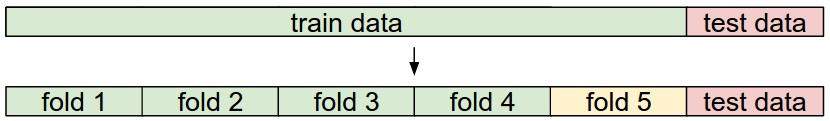
\includegraphics[width=5 in]{pic/crossval}\\
  \caption{Common data splits. A training and test set is given. The training set is split into folds (for example 5 folds here). The folds 1-4 become the training set. One fold (e.g. fold 5 here in yellow) is denoted as the Validation fold and is used to tune the hyperparameters. Cross-validation goes a step further and iterates over the choice of which fold is the validation fold, separately from 1-5. This would be referred to as 5-fold cross-validation. In the very end once the model is trained and all the best hyperparameters were determined, the model is evaluated a single time on the test data (red).}
\end{figure}

\section{Pros and Cons of Nearest Neighbor classifier.}
\begin{itemize}
  \item Pros
      \begin{itemize}
        \item It is very simple to implement and understand. 
        \item It takes no time to train, since all that is required is to store and possibly index the training data.
      \end{itemize}
  \item Cons
    \begin{itemize}
      \item Paying computational cost at test time, since classifying a test example requires a comparison to every single training example. (In practice we often care about the test time efficiency much more than the efficiency at training time. In fact, the deep neural networks we will develop later in this class shift this tradeoff to the other extreme: They are very expensive to train, but once the training is finished it is very cheap to classify a new test example. This mode of operation is much more desirable in practice.)
    \end{itemize}
\end{itemize}

As an aside, the computational complexity of the Nearest Neighbor classifier is an active area of research, and several Approximate Nearest Neighbor (ANN) algorithms and libraries exist that can accelerate the nearest neighbor lookup in a dataset (e.g. \href{http://www.cs.ubc.ca/research/flann/}{FLANN}).

These algorithms allow one to trade off the correctness of the nearest neighbor retrieval with its space/time complexity during retrieval, and usually rely on a pre-processing/indexing stage that involves building a kdtree, or running the $k$-means algorithm.

The Nearest Neighbor Classifier may sometimes be a good choice in some settings (especially if the data is low-dimensional), but it is rarely appropriate for use in practical image classification settings. 
One problem is that images are high-dimensional objects, and distances over high-dimensional spaces can be very counter-intuitive. (See Figure \ref{samenorm})
\begin{figure}
  \centering
  % Requires \usepackage{graphicx}
  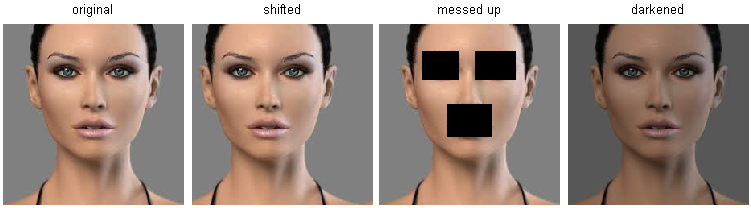
\includegraphics[width=5 in]{pic/samenorm}\\
  \caption{Pixel-based distances on high-dimensional data (and images especially) can be very unintuitive. An original image (left) and three other images next to it that are all equally far away from it based on L2 pixel distance. Clearly, the pixel-wise distance does not correspond at all to perceptual or semantic similarity.}\label{samenorm}
\end{figure}

\section{Applying kNN in practice}
If you wish to apply kNN in practice (hopefully not on images, or perhaps as only a baseline) proceed as follows:
\begin{enumerate}
  \item Preprocess your data: Normalize the features in your data (e.g. one pixel in images) to have zero mean and unit variance. .
  \item If your data is very high-dimensional, consider using a dimensionality reduction technique such as PCA (\href{https://en.wikipedia.org/wiki/Principal_component_analysis}{Wikipedia}) or even \href{http://scikit-learn.org/stable/modules/random_projection.html}{Random Projections}.
  \item Split your training data randomly into train/val splits. As a rule of thumb, between 70-90\% of your data usually goes to the train split.
      \begin{itemize}
        \item More hyperparameters to estimate, larger validation set.
        \item If you are concerned about the size of your validation data, perform cross-validation.
        \item It is always safer to go with cross-validation (the more folds the better, but more expensive).
      \end{itemize}
  \item Train and evaluate the kNN classifier on the validation data (for all folds, if doing cross-validation) for many choices of k (e.g. the more the better) and across different distance types (L1 and L2 are good candidates)
  \item If your kNN classifier is running too long, consider using an Approximate Nearest Neighbor library (e.g. FLANN) to accelerate the retrieval (at cost of some accuracy).
  \item Take note of the hyperparameters that gave the best results. There is a question of whether you should use the full training set with the best hyperparameters, since the optimal hyperparameters might change if you were to fold the validation data into your training set (since the size of the data would be larger). In practice it is cleaner to not use the validation data in the final classifier and consider it to be burned on estimating the hyperparameters. 
  \item Evaluate the best model on the test set. Report the test set accuracy and declare the result to be the performance of the kNN classifier on your data.
\end{enumerate}



